\documentclass[tikz,border=2pt]{standalone}
\usepackage{pgfplots}
\usetikzlibrary{shapes.geometric, intersections}
\pgfplotsset{compat=1.7}

\begin{document}
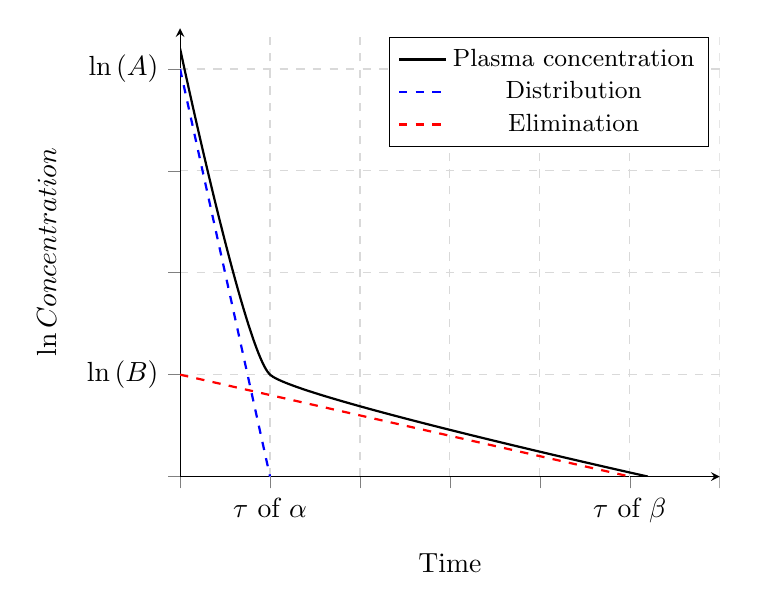
\begin{tikzpicture}

    \begin{axis}[
axis x line=bottom,
  axis y line=left,
	ymin = 0,
	ymax = 2.2,
	xmin = 0,
xmax = 3,
        grid = major,
        grid style={dashed, gray!30},
	 ylabel near ticks,
	xlabel near ticks,
        xlabel=Time,
        ylabel=$\ln{Concentration}$,
	xticklabels={},
	yticklabels={},
        tick align=outside,
        enlargelimits=false,
legend style={font=\small, cells={align=left}},
	extra y ticks={0.5,2},
	extra y tick labels={$\ln{(B)}$,$\ln{(A)}$},
	extra x ticks={0.5,2.5},
	extra x tick labels={$\tau$ of $\alpha$, $\tau$ of $\beta$}]

\draw[black, thick] plot[smooth,tension=0.2] coordinates { (axis cs: 0,2.1) (axis cs: 0.5,0.5) (axis cs: 2.6,0)};
\addlegendimage{black, thick};
\addlegendentry{Plasma concentration}
\addplot[blue,dashed,thick, domain=0:0.5] {2-4*x};
\addlegendentry{Distribution};
\addplot[red,dashed,thick, domain=0:2.5] {0.5-0.2*x};
\addlegendentry{Elimination};




\end{axis}

\end{tikzpicture} 
\end{document}